\chapter{Metode Penelitian}
Pada bab ini disajikan detail perancangan metode penelitian yang perlu dan sangat berpeluang untuk dilakukan dalam rangka menjawab sejumlah permasalahan utama yang diangkat meliputi deskripsi set data publik yang akan digunakan, tahap-tahap pelaksanaan eksperimen dalam berbagai skenario yang diusulkan, metode serta metrik yang digunakan dalam evaluasi dan alat serta bahan penelitian yang diperlukan.

\section{Perancangan Penelitian}
Perancangan penelitian merupakan gambaran utuh mengenai tahap-tahap kerja penulis dalam menemukan solusi permasalahan yang diangkat sebagaimana yang ditunjukkan pada Gambar \ref{fig:desaineksperimen}.
\begin{figure}
    \centering
    \includegraphics[width=14cm]{gambar/alur_penelitian.png}
    \caption{Alur Penelitian}
    \label{fig:desaineksperimen}
\end{figure}

\subsection{Perumusan Masalah}
Beranjak dari penentuan bidang penelitian (\textit{problem area}) yang ditekuni dan penemuan masalah (\textit{problem finding}) yang muncul ---akibat adanya kesenjangan antara harapan dan kenyataan; sebagai bahan utama dalam latar belakang penelitian--- maka selanjutnya masalah tersebut diuraikan dengan berpijak kepada penelitian-penelitian terdahulu. Tahap ini memiliki peran yang sangat penting karena mendasari atas pelaksanaan penelitian.

Dengan perumusan masalah ini akan menghasilkan deskripsi tujuan dan manfaat penelitian secara jelas. Tujuan yang dimaksud adalah keberhasilan penelitian dalam menemukan usulan solusi yang tepat atas permasalahan yang  telah dirumuskan. Sedangkan manfaat yang dimaksud menjelaskan bagaimana penelitian ini dapat berkontribusi kepada kehidupan masyarakat.

\subsection{Studi Literatur}
Tahap ini mencakup usaha peneliti dalam memahami akar dari rumusan masalah yang dihadapi dan mempelajari bagaimana penelitian-penelitian terdahulu dalam menyelesaikan persoalan terkait. Dengan memahami akar permasalahan, peneliti mengetahui teori-teori dan/atau konsep-konsep yang harus dikuasai untuk memulai penelitian. Dengan mempelajari penelitian terkait, peneliti mengetahui wilayah kontribusinya pada bidang penelitian yang sama untuk membuat usulan solusi baru.

Dengan studi literatur ini, penulis dapat memilih untuk mengembangkan solusi yang diusulkan oleh penelitian lain atau mengembangkan solusi baru dalam menyelesaikan persoalan yang sama. Juga penulis dapat mengevaluasi seberapa andal, akurat dan efektif solusi yang diusulkan terhadap penelitian terdahulu. Adapun literatur yang dijadikan sebagai studi berkenaan dengan teori, konsep atau teknik \textit{facial expression recognition}, \acrshort{gcns}, \textit{facial region segmentation} serta berbagai disiplin ilmu terkait lain.

\subsection{Pengumpulan Data}
Pada penelitian ini, penulis menggunakan set data publik FER-2013 diambil dari https://www.kaggle.com/c/challenges-in-representation-learning-facial-expression-\\recognition-challenge/data. Set data ini terdiri dari 35.887 gambar pose wajah yang dilabeli manual berdasarkan tujuh kelas emosi, yaitu \textit{angry}, \textit{disgust}, \textit{fear}, \textit{happy}, \textit{sad}, \textit{surprise}, dan \textit{neutral}. Masing-masing gambar berukuran 48 x 48 piksel dalam skala warna abu-abu (\textit{grayscale}). Pada Gambar \ref{fig:pratinjaufer2013}, diperlihatkan beberapa contoh data gambar FER-2013 per label.
\begin{figure}[ht]
    \centering
    \includegraphics[width=14cm]{gambar/fer2013_label_dist5.png}
    \caption{Pratinjau Set Data FER-2013}
    \label{fig:pratinjaufer2013}
\end{figure}

\begin{figure}[!ht]
    \centering
    \begin{subfigure}[t]{6.75cm}
        \includegraphics[width=6.75cm,height=6.75cm]{gambar/fer2013_label_dist1.png}
        \caption{}
        \label{fig:distribusifer2013a}
    \end{subfigure}
    ~~~
    \begin{subfigure}[t]{6.75cm}
        \includegraphics[width=6.75cm,height=6.75cm]{gambar/fer2013_label_dist4.png}
        \caption{}
        \label{fig:distribusifer2013b}
    \end{subfigure}
    \caption{Distribusi Set Data FER-2013 per Label}
    \label{fig:distribusifer2013}
\end{figure}
Set data ini juga dikelompokkan berdasarkan fungsinya ke dalam set data \textit{training}, \textit{validation} dan \textit{testing} berturut-turut menurut rasio 8{:}1{:}1. Pada Gambar \ref{fig:distribusifer2013a}, diperlihatkan bahwa distribusi data per label tidak merata (\textit{imbalanced dataset}). Yang menjadi kekhawatiran terbesar adalah data berlabel \textit{disgust} hanya ditemukan sejumlah kurang lebih 1,5\% dari keseluruhan. Hal ini dapat menyebabkan model tidak akan mampu mengenali ekspresi wajah \textit{disgust}. Kendati pun demikian, jika mengesampingkan hal tersebut, distribusi set data FER-2013 terbilang cukup merata. Di sisi lain, persebaran data per label untuk tiap-tiap fungsi seimbang sebagaimana yang ditunjukkan oleh Gambar \ref{fig:distribusifer2013b}.

\begin{figure}[htbp]
    \centering
    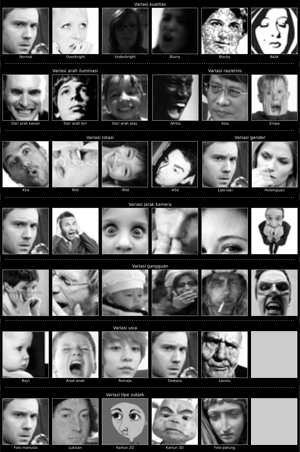
\includegraphics[width=13.7cm]{gambar/fer2013_variasi_all.png}
    \caption{Variasi Set Data FER-2013}
    \label{fig:variasifer2013}
\end{figure}
Disebutkan bahwa set data ini dikumpulkan menggunakan teknik \textit{web crawling} dengan kata kunci terkait emosi, sehingga memiliki variasi yang sangat tinggi terhadap populasi dan lingkungan. Beberapa contoh variasi tersebut ditunjukkan pada Gambar \ref{fig:variasifer2013}. Variasi yang sangat beragam ini penting sekali dalam pertimbangan pemilihan teknik pada sejumlah proses berikutnya meliputi \textit{image enhancement}, \textit{face detection}, \textit{facial landmark detection} dan \textit{facial alignment} yang cocok digunakan.

\subsection{Perancangan Metode}
Pada penelitian ini, penulis memiliki tiga tahap utama sebagaimana yang tertera pada Gambar \ref{fig:rancanganmetode}. Setelah set data FER-2013 dimuat, penulis akan menganalisis apakah terdapat data bising atau tidak. Jika ditemukan data bising atau tidak bersesuaian dengan konteks, maka akan dibersihkan.  Tahap ini disebut \textit{data cleansing} atau \textit{cleaning}. Setelah dibersihkan, maka akan dilakukan penyusunan ulang set data jika diperlukan.
\begin{figure}
    \centering
    \includegraphics[width=14cm]{gambar/perancangan_metode.png}
    \caption{Rancangan Metode}
    \label{fig:rancanganmetode}
\end{figure}

Tahap kedua merupakan praproses data, di mana dilakukan dua skenario penyesuaian sebagaimana yang ditunjukkan oleh Gambar \ref{fig:praprosesdata}. Kedua skenario ini diperlukan berbagai skenario pada tahap ketiga. Pada skenario pertama, praproses hanya melalui tahap \textit{upscaling} ---penyesuaian ukuran dimensi data gambar terhadap arsitektur \acrshort{cnn} yang digunakan--- dan \textit{image enhancement} (jika ada). Pada skenario kedua, ada empat tahap tambahan sebelum pada akhirnya memasuki kedua tahap tadi. Pertama, seluruh data gambar akan dilakukan pendeteksian wajah. Jika terdapat wajah dalam gambar, maka akan diteruskan ke tahap kedua, yaitu pendeteksian \textit{facial landmark}. \textit{Facial landmark} adalah titik-titik koordinat relatif pada setiap gambar yang menunjukkan sekitar komponen wajah seperti mata, hidung dan mulut. Setelah itu, dilakukan penjajaran (\textit{alignment}) area wajah yang terdeteksi terhadap rotasi. Penjajaran yang di sini memiliki dua subtahap, yaitu penjajaran \textit{facial landmark} terhadap \textit{bounding box} dari hasil deteksi wajah dan penjajaran \textit{facial landmark} yang saling bersesuaian. Penjajaran terhadap rotasi ini dihitung menggunakan rumus trigonometri \shortcite{zill2011algebra} pada (\ref{equ:trigonometri}) dengan mengambil tiga titik sampel dari \textit{facial landmark} ---atau dua titik sampel dan sebuah titik hasil pemetaan salah satu dari kedua titik tersebut---,
\begin{equation}
    \theta = \tan^{-1}{\left(\frac{a}{b}\right)} = \tan^{-1}{\left(\frac{B_y-C_y}{A_x-C_x}\right)}
    \label{equ:trigonometri}
\end{equation}
% Penjajaran ini mungkin saja akan mengurangi kemampuan model dalam mengenali emosi yang melibatkan rotasi tertentu seperti yang disebutkan oleh \shortciteA{elfaramawy2017emotion}.
Sebelum ke tahap keempat, tiap-tiap gambar wajah dilakukan pemotongan menurut \textit{bounding box} yang dihasilkan dan perhitungan ulang \textit{facial landmark}. Terakhir, akan dilakukan segmentasi bagian-bagian wajah untuk tiap-tiap gambar berdasarkan \textit{facial landmark} yang dihasilkan.
\begin{figure}
    \centering
    \includegraphics[width=14cm]{gambar/praproses_data.png}
    \caption{Subtahap Praproses Data}
    \label{fig:praprosesdata}
\end{figure}

% TODO: pseudo-code untuk face alignment dan facial region segmentation

Tahap ketiga merupakan tahap eksekusi empat buah skenario pemodelan pengenalan ekspresi wajah. Seperti yang tercantum pada Gambar \ref{fig:skenariotraining}, dua skenario awal merupakan implementasi dan pengembangan model \textit{baseline} dengan mengadopsi ide dari arsitektur \acrshort{gcns} tanpa melibatkan set data hasil dari proses \textit{facial region segmentation}. Skenario berikutnya merupakan pengembangan model terbaik sebelumnya menjadi \textit{network ensemble}. Dilanjutkan dengan skenario terakhir, yaitu uji coba penggantian filter Gabor yang diadopsi pada arsitektur \acrshort{gcns} menjadi filter log-Gabor.
\begin{figure}
    \centering
    \includegraphics[width=14cm]{gambar/skenario_training.png}
    \caption{Subtahap Eksekusi Empat Skenario Pemodelan}
    \label{fig:skenariotraining}
\end{figure}

\subsection{Pengembangan Metode}
Hasil rancangan metode penelitian akan mengalami pengembangan melalui lima tahap prosedur. Tahap pertama, verifikasi terhadap metode penelitian akan dilakukan sebelum metode tersebut diterapkan. Verifikasi ini akan menilai apakah setiap persyaratan teknis dan teoretis yang ditentukan telah dipenuhi atau tidak. Setelah berhasil diverifikasi, metode penelitian akan dieksekusi untuk pertama kalinya.

Tahap kedua merupakan validasi awal terhadap penerapan pertama kali atas metode penelitian. Proses validasi ini akan melibatkan hasil eksperimen dari berbagai literatur yang menjadi rujukan penelitian ini.

Tahap ketiga merupakan inisialisasi konfigurasi pemodelan pengenalan ekspresi wajah seperti menentukan metrik pengukuran yang cocok untuk kasus klasifikasi emosi manusia, menentukan fungsi aktivasi lapisan keluaran yang cocok untuk klasifikasi multikelas, menentukan \textit{seed} untuk beberapa proses yang melibatkan \textit{random number generator}, menentukan berapa kali nilai bobot pada model akan diperbarui ketika \textit{training}, menentukan kapan model perlu disimpan ketika \textit{training} dan menentukan teknik pengukuran kinerja model untuk evaluasi.

Tahap keempat merupakan perbaikan atas metode penelitian yang diusulkan jika pada tahap kedua ditemukan adanya kekurangan atau kesalahan dalam implementasi. Perbaikan ini tidak terbatas pada metode-metode yang telah direncanakan sebelumnya. Melainkan fleksibel mengikuti hasil eksperimen dan hipotesis yang akan muncul dari setiap tahap eksperimen yang dilalui. Metode yang sudah diperbaiki selanjutnya akan dijalankan dan divalidasi kembali.

Setelah metode penelitian telah dinyatakan valid, pada tahap kelima, metode akan dievaluasi dan dioptimalkan berulang kali mengacu pada performa model prediksi yang dihasilkan. Model yang paling optimal akan diambil sebagai hasil akhir dari penelitian ini. Setiap perubahan terkendali pada pengembangan metode ini akan selalu dicatat pada bab berikutnya sebagai bahan evaluasi akhir.

\subsection{Evaluasi Sistem}
Evaluasi sistem dilakukan untuk menyimpulkan performa model pengenalan ekspresi wajah untuk tiap-tiap skenario yang berhasil dieksekusi. Kinerja model diukur menggunakan \textit{f1-score} \shortcite{goutte2005probabilistic} pada (\ref{equ:precision})--(\ref{equ:f1score}),
\small
\begin{equation}
    \text{Precision} = \frac{\text{True Positive}}{\text{True Positive}+\text{False Positive}} = \frac{\text{True Positive}}{\text{Total Predicted Positive}}
    \label{equ:precision}
\end{equation}
\begin{equation}
    \text{Recall} = \frac{\text{True Positive}}{\text{True Positive}+\text{False Negative}} = \frac{\text{True Positive}}{\text{Total Actual Positive}}
    \label{equ:recall}
\end{equation}
\begin{equation}
    \text{F-1 Score} = \frac{2\times\text{Precision}\times\text{Recall}}{\text{Precision}+\text{Recall}}
    \label{equ:f1score}
\end{equation}
\normalsize
\textit{Precision} memberikan gambaran mengenai proporsi identifikasi positif yang benar, sehingga akan bernilai sama dengan 1,0 jika tidak ada \textit{false positive} (kesalahan prediksi pada kelas positif). Sementara \textit{recall} memberikan gambaran mengenai proporsi positif aktual yang diidentifikasi dengan benar, sehingga akan bernilai sama dengan 1,0 jika tidak ada \textit{false negative} (kesalahan prediksi pada kelas negatif). Log pengukuran performa model untuk setiap \textit{epoch} saat \textit{training} juga akan disimpan. Di akhir, evaluasi juga akan dilakukan melalui analisis secara kualitatif.

% TODO: ganti f1-score ke confusion matrix

\section{Alat dan Bahan Penelitian}
Alat yang digunakan pada penelitian ini adalah seperangkat komputer untuk melatih model pengenalan ekspresi wajah. Spesifikasi perangkat keras dan lunak yang digunakan ditunjukkan berturut-turut pada Tabel \ref{tab:spesifikasiperangkatkeras} dan Tabel \ref{tab:spesifikasiperangkatlunak}. Sistem operasi yang digunakan adalah Fedora 32 (\textit{Workstation Edition}) dengan kernel Linux 5.7.8-200. Sementara bahan yang digunakan adalah set data publik pengenalan ekspresi wajah nonfrontal, FER-2013.
\begin{table}
    \caption{Spesifikasi Perangkat Keras}
    \label{tab:spesifikasiperangkatkeras}
    \begin{tabular}{|C{2.7cm}|c|c|c|c|}
        \hline
        Jenis Komponen & \multirow{2}{*}{Merek} & \multirow{2}{*}{Memori} & \multirow{2}{*}{Kecepatan} \\
        \hline\hline
        CPU & Intel Core i5-8250U & - & 1,6GHz--3,4GHz \\
        \hline
        RAM & Corsair Vengeance DDR4 & 2 $\times$ 8GB & 2.400MHz \\
        \hline
        GPU & Nvidia GeForce GTX 1050M & 4GB & - \\
        \hline
    \end{tabular}
\end{table}
\begin{table}
    \caption{Spesifikasi Perangkat Lunak}
    \label{tab:spesifikasiperangkatlunak}
    \begin{tabular}{|C{3.625cm}|C{2.45cm}||C{3.625cm}|C{2.45cm}|}
        \hline
        Nama Program & Versi & Nama Program & Versi \\
        \hline\hline
        CUDA \textit{driver} & 10.2 & jupyter-client & 6.1.3 \\
        \hline
        Nvidia \textit{driver} & 440.100 & LogGabor & 20191113 \\
        \hline
        Visual Studio Code & 1.47.1 & matplotlib & 3.2.1 \\
        \hline
        Python & 3.8.3 & notebook & 6.0.3 \\
        \hline
        GCC & 10.1.1-1 & numpy & 1.18.5 \\
        \hline
        gcn & 1.0 & opencv-python & 4.2.0.34 \\
        \hline
        imgaug & 0.4.0 & pandas & 1.0.4 \\
        \hline
        jupyter & 1.0.0 & scikit-learn & 0.23.1 \\
        \hline
        jupyter-core & 4.6.3 & torch & 1.5.0 \\
        \hline
    \end{tabular}
\end{table}
